\documentclass[10pt]{jarticle}

\usepackage[dvipdfmx]{graphicx}
\usepackage{here}
\title{株式会社 ALBERT 入社課題レポート}
\author{千枝睦実}
\date{2019/03/07}

\begin{document}
\maketitle
\section{課題}
出題された課題は以下の通りである.
本レポートでは,課題5に該当するモデルの構造やハイパーパラメータ,精度について考察とともに述べる.
\begin{enumerate}
\item Linear層,ReLU 関数からなる3層のニューラルネットワークを定義せよ.
ニューラルネットワークの出力は 64次元のベクトルとなるようすること.
\item Triplet lossを用いて1で定義したモデルを訓練せよ.
その際,正常品と正常品および不良品と不良品の間の距離は小さく,正常品と不良品の間の距離は大きくなるようすること.
同時に,異なる不良タイプ(数字)間の距離も大きくなるようにせよ.
Triplet loss の margin は適当に調節すること.
\item 訓練されたモデルを使い,評価セット中のそれぞれのサンプルについて不良度を推定せよ.
学習データ中の正常品を用いて基準となるベクトルを作成し,その基準ベクトルからの距離を不良度とすること.
\item モデルを評価せよ.
評価指標としては,Recall ≥ 0.999を満たす検出閾値を設定した場合の True Negative Rate(真陰性率)を用いること.
\item 作成したモデルの構造やハイパーパラメータ,精度等をレポートにまとめよ.
また,上記設問に従って作成したモデルの欠点を指摘し,改善案を自由に記述せよ.
\end{enumerate}

\section{開発環境}
開発に使用した環境を表\ref{env}に示す。
このうち、matplotlibは本レポートにある図表の作成にのみ使用した。
\begin{table}[H]
\caption{開発環境}
\label{env}
\centering
\begin{tabular}{ccrr} \hline
種別 & 名称 & バージョン & 備考 \\ \hline
OS & Windows & 10 ビルド17134.590 & - \\
CPU & Intel Core i7-4790 CPU 8GB & - & 3.6GHz \\
GPU & GeForce GTX 1060 6GB & - & - \\ 
言語 & Python & 3.7.1 & - \\
モジュール & CUDA & v10.1 & - \\
 & cupy & 5.3.0 & ビルド100010 \\
 & numpy & 1.16.2 & - \\
 & chainer & 5.3.0 & - \\
 & matplotlib & 3.0.3 & - \\ \hline
\end{tabular}
\end{table}

\section{モデル構造}
作成したモデルの構造を図\ref{nn}に示す.
課題1に示された通り,3層のLinear層でニューラルネットワークを形成し,ユニットによる次の層への出力にはReLU関数を用いた.

\begin{figure}[H]
  \centering
  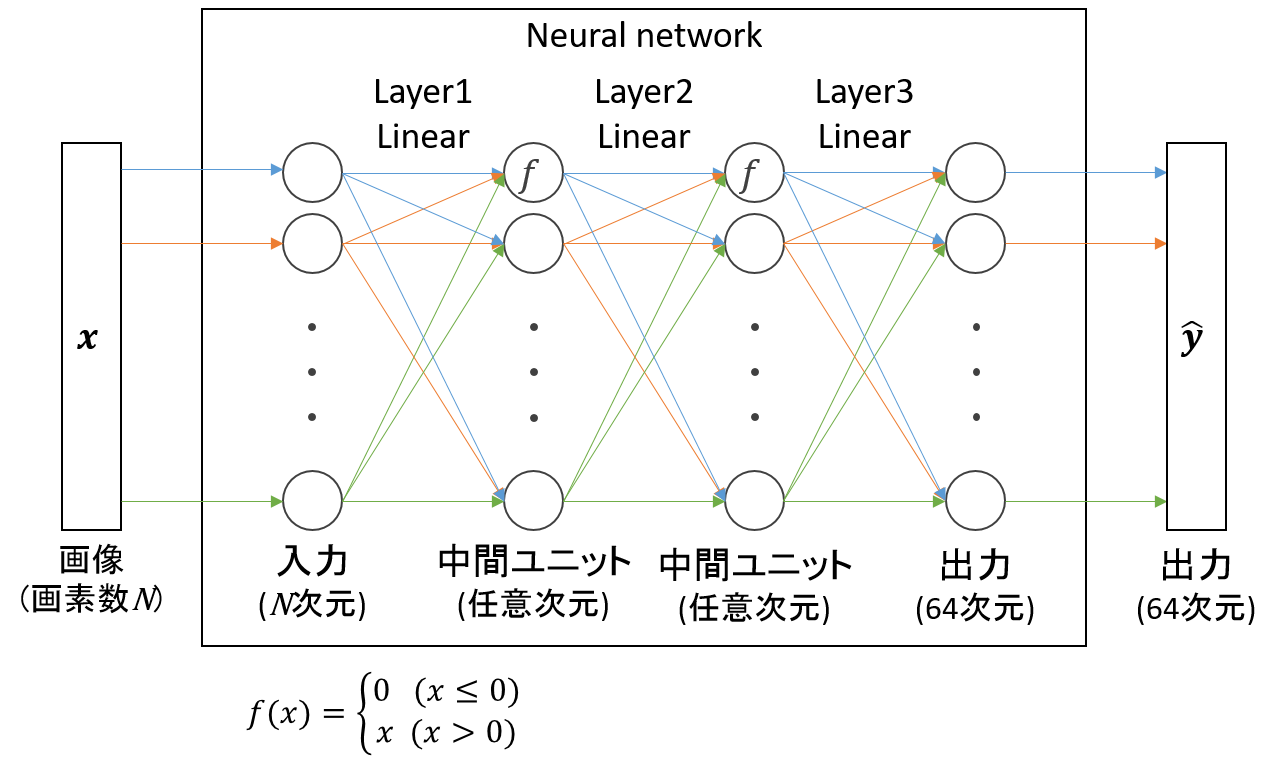
\includegraphics[width=12cm]{nn.png}
  \label{nn}
  \caption{作成したモデルの構造}
\end{figure}

今回の課題では,テストケースにある未知の値に対応するためTriplet loss関数を用いた距離学習を行う.
そこで,各サンプルに対するトリプレットを予め作成しておき,訓練データとした.
したがって,作成したモデルは訓練データのトリプレットロスを最小化するように各サンプルに対して距離学習する.\\
\quad その後,正常画像(0,6,9)の基準ベクトルを作成し,基準ベクトルとの距離が検知閾値以上のものを異常画像とした.
検知閾値は0から大きくしていき,Recall$\ge $0.999を満たさなくなった時点で最も大きい真陰性率(selectivity)を出した閾値を採用し,最終的な予測を出力する.

\section{モデルの評価}
モデルのハイパーパラメータの初期値を表\ref{1stparams}に示す.
なお,エポック数は50に設定しているが,Early stoppingを導入しているため,実際はこれよりもエポック数は少なくなる.

\begin{table}[H]
\caption{各ハイパーパラメータの初期値}
\label{1stparams}
\centering
\begin{tabular}{rr} \hline
ハイパーパラメータ & 値 \\ \hline
最適化アルゴリズム & SGD \\
中間層ユニット数 & 256 \\
ミニバッチ数 & 100 \\
Triplet loss関数のマージン & 0.2 \\ \hline
\end{tabular}
\end{table}

このパラメータで学習したモデルによるRecall $\ge$ 0.999時の最大真陰性率は,0.06719であり,エポック数は46だった.\\
\quad ここで,検出閾値ごとのRecallと真陰性率を図\ref{tnrateInit}に示す.
Recall$\ge$ 0.99だった場合の真陰性率は0.32440,Recall$\ge$ 0.9だった場合の真陰性率は0.78792であった.
そのため,学習・予測自体は正常に行われていると判断し,ここからはハイパーパラメータ探索で改善する.

\begin{figure}[H]
  \centering
  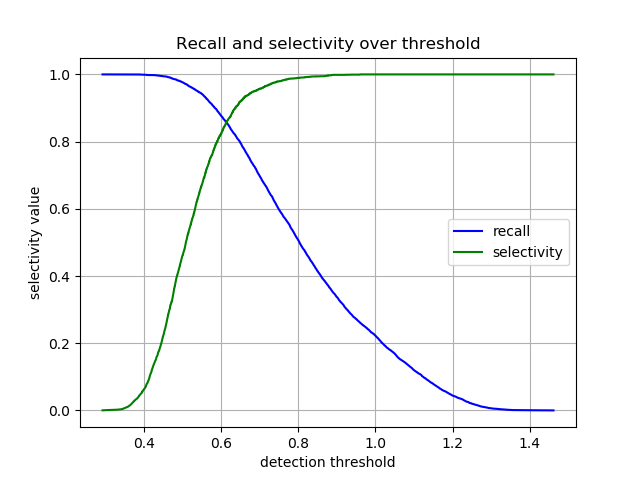
\includegraphics[width=12cm]{tnrate_init.png}
  \label{tnrateInit}
  \caption{検出閾値ごとのRecallと真陰性率}
\end{figure}

\subsection{アルゴリズム比較}
まず,最適化アルゴリズムの検討を行った.
各アルゴリズムを用いたときの,Recall $\ge$ 0.999における真陰性率を表\ref{algorithm}に示す.
この中で,CorrectedMomentumSGDアルゴリズムを用いたモデルが,最も高い真陰性率(0.19206)を出した.
そこで,その他のパラメータはこのアルゴリズムを用いたモデルで探索する.
また,このうち,AdaDelta,Adam,RMSprop,SMORMS3アルゴリズムでは,テストケースでのTriplet lossがエポックごとに増大していったため,どれも4回のエポックでEarly stoppingが行われた.
原因については,期間の関係で検証できなかった.
\begin{table}[H]
\centering
\caption{最適化アルゴリズムと真陰性率}
\label{algorithm}
\centering
\begin{tabular}{rr} \hline
アルゴリズム & 真陰性率 \\ \hline
AdaDelta & 0.05327 \\ %4 テストのロスが収束しない
AdaGrad & 0.08042 \\ %7
Adam & 0.05836 \\ %4 テストのロスが収束しない
CorrectedMomentumSGD & 0.19206 \\ %10
NesterovAG & 0.12080 \\ %8
RMSprop & 0.02681 \\ %4 異常に大きいロス
RMSpropGraves & 0.09874 \\ %7
SGD & 0.06719 \\ %46
SMORMS3 & 0.04309 \\ \hline %4 
\end{tabular}
\end{table}

\subsection{Triplet lossのマージン}
次に,アルゴリズムを真陰性率の高かったCorrectedMomentumアルゴリズムに変更し,最適なTriplet lossのマージンを探索する.
マージンの,各値でのRecall $\ge$ 0.999における真陰性率を表\ref{margin}に示す.
マージンが0.3の時に,最も高い真陰性率(0.20835)を出した.
\begin{table}[H]
\centering
\caption{Triplet loss関数のマージンと真陰性率}
\label{margin}
\begin{tabular}{rr} \hline
マージン & 真陰性率 \\ \hline
0.01 & 0.10757  \\ %10
0.1 & 0.19206 \\ %10
0.2 & 0.19206 \\ %10
0.25 & 0.16050 \\ %7
0.3 & 0.20835 \\ %9
0.35 & 0.11503 \\ %5
0.4 & 0.14388 \\ \hline %7
\end{tabular}
\end{table}

\subsection{中間層のユニット数}
マージンを0.3に変更し,中間層のユニット数を探索する.
中間層のユニット数の,各値でのRecall $\ge$ 0.999における真陰性率を表\ref{mid}に示す.
中間層のユニット数が256の時に,最も高い真陰性率(0.20835)を出した.
\begin{table}[H]
\centering
\caption{中間層のユニット数と真陰性率}
\label{mid}
\begin{tabular}{rr} \hline
ユニット数 & 真陰性率 \\ \hline
64 & 0.05701  \\ 
128 & 0.00441 \\
200 & 0.06481 \\
255 & 0.08551 \\
256 & 0.20835 \\
257 & 0.08483 \\
300 & 0.04208 \\
400 & 0.06820 \\
512 & 0.06108 \\
1024 & 0.09773 \\ \hline
\end{tabular}
\end{table}

\subsection{ミニバッチサイズ}
中間層のユニット数を256に変更し,ミニバッチサイズを探索する.
ミニバッチサイズの各値でのRecall $\ge$ 0.999における真陰性率を表\ref{batch}に示す.
ミニバッチサイズが100の時に,最も高い真陰性率(0.20835)を出した.
\begin{table}[H]
\centering
\caption{ミニバッチサイズと真陰性率}
\label{batch}
\begin{tabular}{rr} \hline
ユニット数 & 真陰性率 \\ \hline
10 & 0.002850  \\ 
50 & 0.19545 \\
95 & 0.16661 \\
99 & 0.18681 \\
100 & 0.20835 \\
101 & 0.18867 \\
105 & 0.12182 \\
120 & 0.18697 \\
150 & 0.16254 \\
200 & 0.19104 \\
300 & 0.14048 \\
400 & 0.06820 \\
500 & 0.16966 \\
1000 & 0.17374 \\ \hline
\end{tabular}
\end{table}

\subsection{探索結果}
今回のハイパーパラメータ探索で得られた結果を表\ref{total}に示す.
このパラメータで得られたRecall $\ge$ 0.999における真陰性率は0.20835であった.
本レポートでは,各パラメータを順番に調整したが,本来であれば,グリッドサーチや,optunaライブラリによるパラメータ最適化の方法を用いるべきであると考えられる.
\begin{table}[H]
\caption{探索で得られたハイパーパラメータ}
\label{total}
\centering
\begin{tabular}{rr} \hline
ハイパーパラメータ & 値 \\ \hline
最適化アルゴリズム & CorrectedMomentumSGD \\
中間層ユニット数 & 256 \\
Triplet loss関数のマージン & 0.3 \\ 
ミニバッチ数 & 100 \\ \hline
\end{tabular}
\end{table}


\section{考察}
\subsection{モデルの欠点}
今回の課題では,使用するニューラルネットワークは全結合層が3層の構成であった.\\
\quad 全結合層の問題点として,情報を1次元のベクトルとして入出力するため,画像を認識する際,空間的な位置情報が無視される点が挙げられる.
たとえば,64画素の画像で,$(x,y) = (1,2)$の画素と$(x,y) = (1,3)$の画素は隣りあっているが,全結合層では$x = 9$の画素と$x = 17$の画素として扱われ,隣接していたという情報が失われている.\\
\quad また,全結合層は,接続数が多く,必要な計算量や勾配消失の観点から,今日よく使われる高画質な画像には対応できない点も挙げられる.\\

\subsection{改善案}
\begin{enumerate}
\item 画像認識では,特徴抽出を行う畳み込み層と,物体の位置の違いを吸収するプーリング層とを交互に配置した畳み込みニューラルネットワーク(CNN)が適するとされている.
その理由として,以下の点が挙げられる.
\begin{itemize}
\item 畳み込み層の複数のフィルタによって,画像のサイズごと,部分ごとの特徴を保持できる.
\item プーリング層による圧縮によって,物体の位置の微少なずれに影響されにくい.
\end{itemize}
そこで,今回のモデルの代わりにCNNを使用して学習するという案が考えられる.
\item 異常とする画像が訓練データに少なく,十分に学習できなかった可能性が考えられる.
そこで,異常なサンプルをアフィン変換や射影変換などで変換したものを訓練データに加えて学習する方法が考えられる.

\item ハイパーパラメータの探索が不十分だった可能性が考えられる.
そこで,optunaなどのライブラリを用いて最適なパラメータを求めた上で学習する方法が考えられる.
\end{enumerate}

\end{document}